% ======================= ANEXOS =======================
% Numeración de tablas y figuras por anexo (A1, B1, C1...), como en la etapa 3.
\newcommand{\iniciaanexo}[1]{%
  \setcounter{table}{0}\setcounter{figure}{0}%
  \renewcommand{\thetable}{#1\arabic{table}}%
  \renewcommand{\thefigure}{#1\arabic{figure}}}

% ----------------------- ANEXO A -----------------------
\anexo{Anexo A. Técnicas no exitosas o no adoptadas}
\iniciaanexo{A}
La Tabla~\ref{tbl:a-noexitosas} distingue las alternativas evaluadas de las que solo se consideraron.

\begin{table}[H]
\centering\footnotesize
\caption{Técnicas que se probaron o se consideraron y no se adoptaron, con su resultado y la razón.}
\label{tbl:a-noexitosas}
\begin{tabularx}{\textwidth}{>{\raggedright\arraybackslash}p{3.0cm}>{\raggedright\arraybackslash}p{3.4cm}>{\raggedright\arraybackslash}p{3.8cm}L}
\toprule
Técnica & Qué se hizo & Resultado & Por qué no se adoptó\\
\midrule
Conglomerados para regímenes multicontaminante (etapa 1) & Propuesta de la etapa 1: agrupar días por la combinación de seis contaminantes & No se llegó a ajustar & La retroalimentación pidió acotar el problema; se reenfocó en el PM2.5\\
Componentes principales como predictores de M1 & M1 con PC1–PC3 en lugar de las 8 variables (etapa 3) & \dauc{} 0.064 [0.039, 0.090] frente a 0.070 & Los componentes maximizan la varianza, no la separación, y mezclan efectos opuestos\\
Interacción estación × temporada & M0 y M1 con la interacción (etapa 3) & \dauc{} 0.056 [0.036, 0.076] frente a 0.070 & No cambia la conclusión y duplica los parámetros\\
Transformaciones logarítmicas (lluvia y viento) & Validación progresiva en 2021–2023 (etapa 3) & AUC +0.003 y +0.007 en la validación & Mejora mínima; el logaritmo sobrecorregía la asimetría del viento\\
QDA (regularizada y sin regularizar) & Misma partición que el LDA (base v2) & AUC 0.788 frente a 0.792 (todos los predictores); 0.704–0.712 frente a 0.718 (solo meteorología) & Estima muchos más parámetros; ganar en supuestos no se tradujo en mejor clasificación\\
MICE para la imputación diaria & Enmascaramiento diario en 2021–2023 (base v2) & RMSE relativo 0.436 (promedio de 5 imputaciones) y 0.593 (una base) frente a 0.450 de la mediana ajustada; como sensibilidad, \dauc{} 0.078 & Casi empatado en error puntual; se prefirió la mediana ajustada por ser determinista y simple, y MICE queda como sensibilidad\\
Aprendizaje profundo para imputar (MIMA-v1) & Revisión del método y solicitud de su dataset imputado & Sin acceso al dataset imputado a tiempo & No se pudo usar; una sensibilidad con su meteorología en sus 9 estaciones, con PM2.5 observado, queda pendiente (Sección~\ref{sec:imputacion})\\
Imputación por vecinos cercanos (KNN) & No se aplicó & — & No se aplicó en esta etapa, siguiendo la retroalimentación del curso. Un KNN que ignore el tiempo y la estructura de la red puede seleccionar donantes poco pertinentes; existen variantes que incorporan esa información (Belachsen \& Broday, 2022), cuya comparación queda fuera del alcance\\
\bottomrule
\end{tabularx}
\end{table}

% ----------------------- ANEXO B -----------------------
\anexo{Anexo B. Preparación de los datos y diccionario resumido}
\iniciaanexo{B}
Este anexo reúne el detalle de la preparación de los datos que se resume en las Secciones~\ref{sec:area} y~\ref{sec:preparacion}: las estaciones (Tabla~\ref{tbl:estaciones}), los cambios en la red (Tabla~\ref{tbl:b-cambios}), el largo de los huecos (Tabla~\ref{tbl:b-huecos}), la imputación horaria elegida (Tabla~\ref{tbl:imputacion}) y su error (Figura~\ref{fig:imputacion}), las exclusiones por estación, temporada y año (Tabla~\ref{tbl:b-exclusiones}), las reglas de limpieza (Tabla~\ref{tbl:b-limpieza}) y el diccionario (Tabla~\ref{tbl:b-diccionario}).

\begin{table}[H]
\centering\small
\caption{Estaciones de la muestra: altitud, días-estación en el análisis final y porcentaje con PM2.5 > 25\ugm{} (base v2, 2021–2025). Municipio según los metadatos de SIMA; el de NTE2, SE3 y SUR (marcado con *), que no viene en ellos, se completó por la ubicación de la estación. † NO2 incluye el periodo con PM2.5 anómalo frente a la red (Anexo~C).}
\label{tbl:estaciones}
\begin{tabular}{lllrrr}
\toprule
Código & Nombre & Municipio & Altitud (m) & Días-estación & \% superación\\
\midrule
SE2 & Juárez & Juárez & 387 & 1\,680 & 46.1\\
SO & Santa Catarina & Santa Catarina & 674 & 1\,284 & 43.8\\
CE & Obispado & Monterrey & 562 & 1\,555 & 35.3\\
NO & San Bernabé & Monterrey & 568 & 631 & 32.5\\
NE2 & Apodaca & Apodaca & 432 & 1\,215 & 31.2\\
NE & San Nicolás & San Nicolás de los Garza & 474 & 1\,282 & 29.1\\
NTE2 & Universidad & San Nicolás de los Garza* & 520 & 1\,696 & 23.2\\
SE3 & Cadereyta & Cadereyta Jiménez* & 334 & 1\,574 & 19.1\\
SO2 & San Pedro & San Pedro Garza García & 636 & 1\,564 & 18.9\\
NO2† & García & García & 702 & 1\,532 & 18.4\\
SE & La Pastora & Guadalupe & 500 & 1\,287 & 15.3\\
NTE & Escobedo & Escobedo & 503 & 1\,373 & 14.8\\
SUR & Pueblo Serena & Monterrey* & 555 & 1\,155 & 10.6\\
\bottomrule
\end{tabular}
\end{table}

\begin{table}[H]
\centering\footnotesize
\caption{Cambios en la red y anomalías detectadas, y cómo se tomaron en cuenta. Fuentes: PIGECA (SMA y CAI, 2024, p.~91), SIMA (comunicación personal, 9 y 15 de octubre de 2026) y diagnósticos propios.}
\label{tbl:b-cambios}
\begin{tabularx}{\textwidth}{>{\raggedright\arraybackslash}p{3.3cm}LL}
\toprule
Cambio & Detalle & Cómo se tomó en cuenta\\
\midrule
Reubicaciones según el PIGECA & NO (junio de 2021); SE, SO, NTE y SUR (septiembre de 2021); NE (febrero de 2022) & Entrenamiento sin los días previos (D23); en la presión solo se ve el cambio de SUR (+5.7\,mm\,Hg) y algo el de NTE (+1.6)\\
Reubicaciones confirmadas por SIMA & NO, SE, SUR, NE y NO3 (sin fechas); no mencionaron SO ni NTE & Sensibilidad con esta lista: \dauc{} 0.081\\
Sensores de viento nuevos & Todas las estaciones, 2021; el nivel del viento cambia entre marzo y abril de 2021 & Se excluye 2020 del modelado; enero a marzo de 2021 sigue en el entrenamiento con el nivel anterior\\
Equipos de PM2.5 nuevos & SE2, NTE2, SUR, SO2 y NO, 2025 (Thermo 5014i) & Mejora por año: 0.069 (2024) y 0.088 (2025)\\
PM2.5 de NO2 (García) bajo frente a la red & El PM2.5 baja a cerca de la mitad del nivel de la red mientras el PM10 sigue normal: enero–mayo de 2021 y julio de 2023–enero de 2025 & En la prueba, 272 de sus 538 días caen en enero de 2024–enero de 2025, sin ninguna superación (22.6\,\% en los demás); sensibilidad sin NO2: \dauc{} 0.082; pregunta para SIMA\\
Radiación solar muy baja & NO2 y NTE: media de SR de 0.015 y 0.041\,kW/m², frente a 0.12–0.18 en las demás & Sensibilidad con SR imputada ≥ 0: \dauc{} 0.079; pregunta para SIMA\\
\bottomrule
\end{tabularx}
\end{table}

\begin{table}[H]
\centering\small
\caption{Largo de los huecos horarios antes de imputar (13 estaciones, 2021–2025): porcentaje de horas faltantes y reparto de esas horas según el largo del hueco al que pertenecen.}
\label{tbl:b-huecos}
\begin{tabular}{lrrrrrr}
\toprule
Variable & \% faltante & 1–3\,h & 4–6\,h & 7–24\,h & 1–7 días & > 7 días\\
\midrule
PM2.5 & 17.2 & 20.7 & 5.9 & 14.0 & 15.7 & 43.6\\
Temperatura & 6.3 & 9.0 & 3.5 & 13.3 & 12.0 & 62.2\\
Humedad relativa & 10.1 & 6.4 & 2.5 & 9.9 & 9.0 & 72.2\\
Radiación solar & 8.8 & 3.4 & 1.1 & 13.5 & 19.6 & 62.4\\
Presión & 3.7 & 22.9 & 7.5 & 19.0 & 22.1 & 28.5\\
Viento (\emph{u}, \emph{v}) & 6.7 & 12.7 & 4.8 & 15.0 & 19.3 & 48.3\\
\bottomrule
\end{tabular}
\end{table}

\begin{table}[H]
\centering\small
\caption{Imputación horaria de la meteorología elegida por enmascaramiento (2021–2023): método, hueco máximo imputado (maxgap), error medio de la interpolación lineal frente al ganador, porcentaje de imputaciones revertidas por la revalidación y horas imputadas en 2021–2025 (13 estaciones) frente a la etapa 3.}
\label{tbl:imputacion}
\begin{tabularx}{\textwidth}{llrRrr}
\toprule
Variable & Método & maxgap (h) & Error de la lineal frente al ganador & \% revertido & Horas imputadas (etapa 3 → 4)\\
\midrule
Temperatura & Descomposición estacional & 12 & +84.9\,\% & 0.06 & 3\,149 → 5\,800\\
Humedad relativa & Kalman (StructTS) & 6 & +23.1\,\% & 2.51 & 3\,345 → 4\,398\\
Radiación solar & Interpolación de Stineman & 2 & +6.8\,\% & 3.66 & 1\,711 → 1\,473\\
Presión & Descomposición estacional & 12 & +88.6\,\% & 0.00 & 4\,742 → 7\,629\\
Viento \emph{u} & Interpolación lineal & 3 & +0.4\,\% & 0.00 & 4\,793 → 4\,790\\
Viento \emph{v} & Interpolación lineal & 3 & +0.0\,\% & 0.00 & 4\,793 → 4\,790\\
\bottomrule
\end{tabularx}
\end{table}

\begin{figure}[H]
\centering
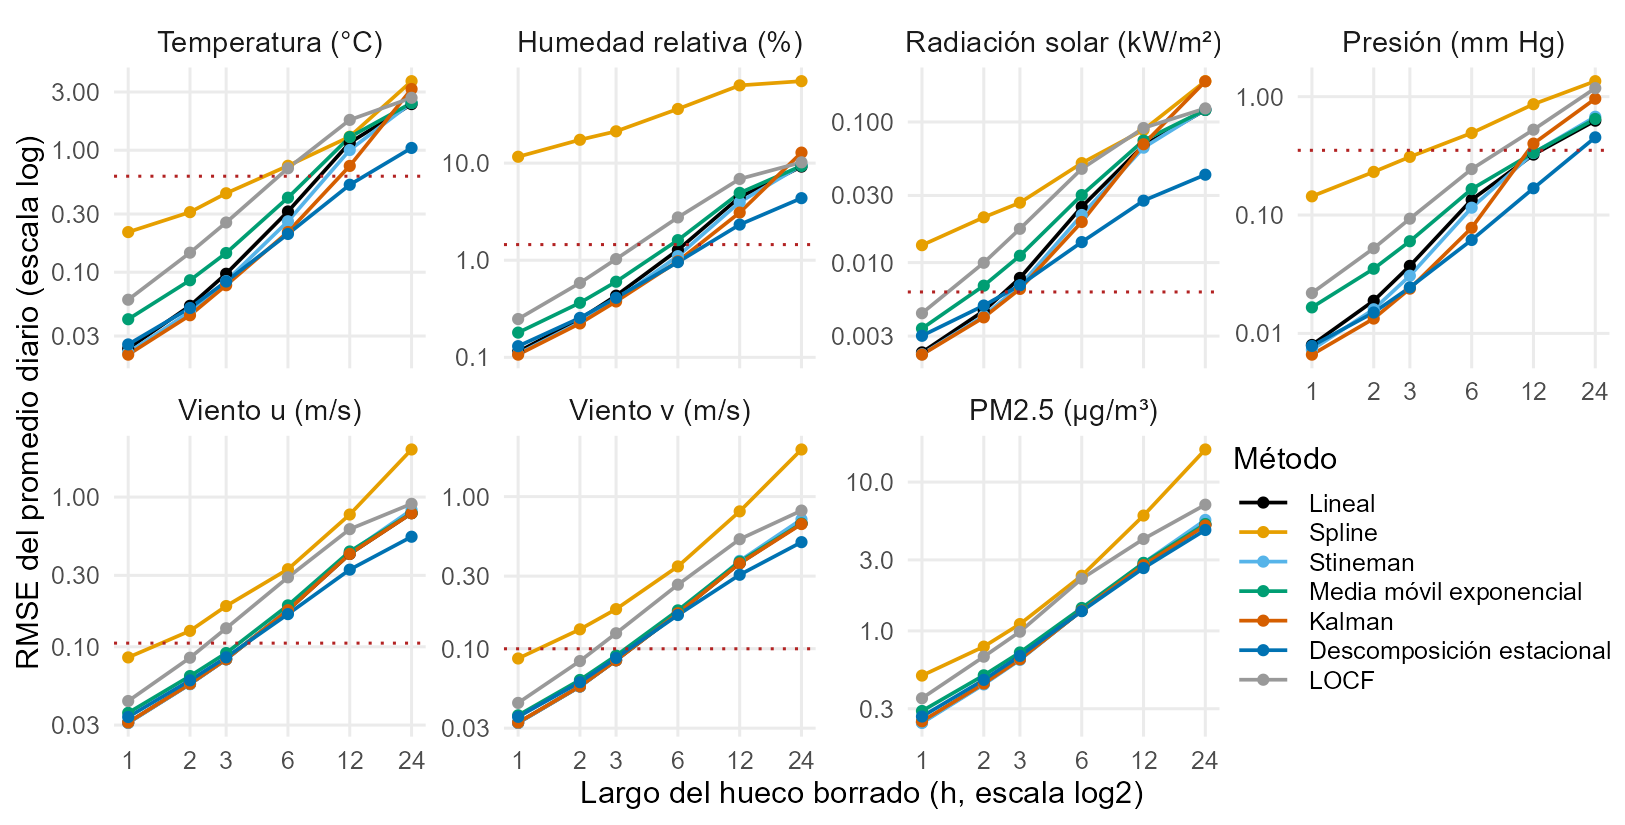
\includegraphics[width=0.95\textwidth]{figuras/rmse_imputacion_informe.png}
\caption{Error (RMSE) del promedio diario según el método de imputación y el largo del hueco borrado, en tramos completos de 2021–2023 (13 estaciones, 5 repeticiones, 2\,730 series por método). Escalas logarítmicas; la línea punteada es el umbral de error tolerado. PM2.5 solo como diagnóstico.}
\label{fig:imputacion}
\end{figure}

La Tabla~\ref{tbl:b-exclusiones} detalla las causas de exclusión que resume la Tabla~\ref{tbl:exclusiones} (Sección~\ref{sec:muestra}).

\begin{table}[H]
\centering\small
\caption{Causas de exclusión por estación, temporada y año (2021–2025): días-estación posibles, sin PM2.5 suficiente (a), con meteorología imputada (c), con 5–8 meteorológicas faltantes (d) y previos a una reubicación (e), y porcentaje de superación en (b) y (c).}
\label{tbl:b-exclusiones}
\begin{tabular}{lrrrrrrr}
\toprule
Grupo & Días posibles & (a) n (\%) & (c) n (\%) & (d) n & (e) n & \% superación (b) & \% superación (c)\\
\midrule
CE & 1\,826 & 268 (14.7) & 100 (5.5) & 3 & 0 & 33.7 & 58.0\\
NE & 1\,826 & 124 (6.8) & 550 (30.1) & 7 & 413 & 29.3 & 27.8\\
NE2 & 1\,826 & 608 (33.3) & 240 (13.1) & 3 & 0 & 33.5 & 21.7\\
NO & 1\,826 & 1\,046 (57.3) & 128 (7.0) & 2 & 147 & 34.8 & 18.8\\
NO2 & 1\,826 & 289 (15.8) & 1\,023 (56.0) & 5 & 0 & 9.8 & 22.7\\
NTE & 1\,826 & 234 (12.8) & 925 (50.7) & 78 & 141 & 18.7 & 16.6\\
NTE2 & 1\,826 & 128 (7.0) & 7 (0.4) & 2 & 0 & 23.3 & 14.3\\
SE & 1\,826 & 285 (15.6) & 148 (8.1) & 22 & 232 & 15.4 & 28.4\\
SE2 & 1\,826 & 140 (7.7) & 206 (11.3) & 6 & 0 & 48.4 & 29.6\\
SE3 & 1\,826 & 249 (13.6) & 337 (18.5) & 3 & 0 & 16.9 & 27.0\\
SO & 1\,826 & 247 (13.5) & 277 (15.2) & 36 & 259 & 46.8 & 33.6\\
SO2 & 1\,826 & 261 (14.3) & 169 (9.3) & 1 & 0 & 20.0 & 9.5\\
SUR & 1\,826 & 467 (25.6) & 82 (4.5) & 21 & 183 & 9.6 & 9.8\\
\midrule
Seca-fría & 7\,813 & 1\,367 (17.5) & 1\,488 (19.0) & 91 & 319 & 38.3 & 34.8\\
Seca-cálida & 5\,980 & 1\,028 (17.2) & 1\,037 (17.3) & 78 & 462 & 36.1 & 29.0\\
Lluvias & 9\,945 & 1\,951 (19.6) & 1\,667 (16.8) & 20 & 594 & 12.8 & 10.0\\
\midrule
2021 & 4\,745 & 596 (12.6) & 1\,186 (25.0) & 99 & 1\,321 & — & —\\
2022 & 4\,745 & 468 (9.9) & 526 (11.1) & 5 & 54 & — & —\\
2023 & 4\,745 & 725 (15.3) & 604 (12.7) & 2 & 0 & — & —\\
2024 & 4\,758 & 1\,118 (23.5) & 843 (17.7) & 1 & 0 & — & —\\
2025 & 4\,745 & 1\,439 (30.3) & 1\,033 (21.8) & 82 & 0 & — & —\\
\bottomrule
\end{tabular}
\end{table}

\begin{table}[H]
\centering\small
\caption{Reglas de limpieza horaria, en el orden en que se aplican, y horas anuladas en las 15 variables (2020–2025). Fuente: \texttt{data/clean/README.md} y \texttt{tabla\_informe\_limpieza.csv}.}
\label{tbl:b-limpieza}
\begin{tabularx}{\textwidth}{>{\raggedright\arraybackslash}p{4.4cm}L>{\raggedleft\arraybackslash}p{2.6cm}}
\toprule
Regla (bandera) & Criterio & Horas anuladas\\
\midrule
Rango duro (F) & Fuera del rango de operación (contaminantes) o del fabricante (meteorología) & 2\,409\\
Notas del PDF de SIMA (P) & Límites anuales que indica SIMA & 116\\
Saturación del sensor (L) & |TOUT| ≥ 49.9\,°C & 25\\
Salto horario (S) & |ΔTOUT| > 10\,°C o |ΔPRS| > 10\,mm\,Hg en una hora & 2\,576\\
PM2.5 > PM10 (R) & Se anulan las dos & 74\\
Racha de valores idénticos (K) & ≥ 24\,h iguales en contaminantes, TOUT, PRS y RH & 13\,598\\
Consistencia espacial, D14 (E) & TOUT a > 10\,°C o RH a > 40\,pp de la mediana de la red (≥ 5 estaciones) & 450 TOUT y 4\,120 RH\\
Radiación de madrugada, D15 (M) & Media de SR entre 00 y 04\,h > 0.02\,kW/m²: se anula todo el día & 49\,491\\
Viento contra la red, D15 (E) & WSR > mediana de la red + 30\,km/h; ≥ 3 horas anulan el día & 4\,426 horas de WSR\\
\bottomrule
\end{tabularx}
\end{table}

Las reglas se aplican en el orden de la Tabla~\ref{tbl:b-limpieza}, sobre los valores horarios observados y antes de imputar. Las horas anuladas por consistencia espacial, saturación o radiación de madrugada nunca se imputan. Todo valor imputado se revalida con las mismas reglas y, si incumple alguna, vuelve a faltante (bandera X); nunca se modifica un valor original válido. La consistencia espacial se repite hasta que ninguna lectura conservada incumple respecto de su propia mediana de la red, y sus umbrales se eligieron con la distribución de las desviaciones y un análisis de sensibilidad (8, 10 y 15\,°C; 30, 40 y 50 puntos porcentuales). El detalle completo, con las cifras por estación, está en \texttt{data/clean/README.md}. La Tabla~\ref{tbl:b-diccionario} resume las variables y sus transformaciones; los diccionarios completos se encuentran en el repositorio.

\begin{table}[H]
\centering\small
\caption{Variables de la base diaria v2 que usa el modelo (\texttt{data/clean/v2/diario\_v2\_imputado\_2021\_2025.csv}).}
\label{tbl:b-diccionario}
\begin{tabularx}{\textwidth}{>{\raggedright\arraybackslash}p{5.4cm}L}
\toprule
Variable & Descripción\\
\midrule
\texttt{estacion}, \texttt{fecha}, \texttt{anio}, \texttt{temporada} & Clave del día-estación y temporada (seca-fría nov–feb, seca-cálida mar–may, cálida-húmeda o lluvias jun–oct)\\
\texttt{PM2.5} & Media diaria con ≥ 18\,h observadas (µg/m\textsuperscript{3}); no se imputa\\
\texttt{supera\_25} & 1 si PM2.5 > 25\ugm{} (referencia fija)\\
\texttt{TOUT}, \texttt{RH}, \texttt{SR}, \texttt{PRS} & Media diaria de temperatura (°C), humedad (\%), radiación (kW/m²) y presión (mm\,Hg)\\
\texttt{viento\_u}, \texttt{viento\_v}, \texttt{viento\_rapidez\_ms} & Componentes y rapidez media diaria del viento (m/s)\\
\texttt{horas\_lluvia} & Horas del día con lluvia (0–24)\\
\texttt{imp\_TOUT}, \texttt{imp\_RH}, … (una por variable) & 1 si la variable de ese día se imputó a nivel diario\\
\texttt{sitio\_valido} & 0 en los días previos a la reubicación de la estación (D23)\\
\bottomrule
\end{tabularx}
\end{table}

% ----------------------- ANEXO C -----------------------
\anexo{Anexo C. Diagnósticos complementarios}
\iniciaanexo{C}
La Tabla~\ref{tbl:puente} detalla el paso de la etapa 3 a la etapa 4 (Sección~\ref{sec:validacion}), y la Tabla~\ref{tbl:robustez}, las variantes de la Sección~\ref{sec:robustez}.

\begin{table}[H]
\centering\small
\caption{Tabla puente de la etapa 3 (datos-v1.2) al análisis final de la etapa 4 (base v2): tamaño de entrenamiento y de prueba, porcentaje de superación en la prueba, AUC de M0 y M1 y \dauc{} con IC 95\,\% (bootstrap por bloques de 14 días, 1\,000 réplicas).}
\label{tbl:puente}
\begin{tabularx}{\textwidth}{cLrrrrr}
\toprule
Paso & Cambio & n entren. / prueba & \% sup. & AUC M0 & AUC M1 & \dauc{} [IC 95\,\%]\\
\midrule
0 & Etapa 3 (datos-v1.2) & 10\,170 / 5\,220 & 27.2 & 0.722 & 0.792 & 0.070 [0.047, 0.094]\\
1 & + respuesta solo con horas observadas (D18) & 9\,983 / 4\,978 & 28.3 & 0.716 & 0.790 & 0.074 [0.051, 0.098]\\
2 & + imputación horaria de la meteorología (D19) & 10\,024 / 4\,987 & 28.4 & 0.717 & 0.790 & 0.074 [0.050, 0.098]\\
3 & + imputación diaria con la mediana de la red ajustada (D20) & 12\,340 / 6\,863 & 26.2 & 0.709 & 0.791 & 0.081 [0.055, 0.109]\\
4 & + entrenamiento sin días previos a la reubicación (D23) = análisis final & 10\,965 / 6\,863 & 26.2 & 0.713 & 0.792 & 0.079 [0.054, 0.104]\\
\bottomrule
\end{tabularx}
\end{table}

\begin{table}[H]
\centering\small
\caption{\dauc{} (M1 − M0) en la prueba 2024–2025 según el análisis, con IC 95\,\% por bootstrap por bloques de 14 días salvo que se indique. Las cuatro últimas filas son sensibilidades posteriores a la evaluación; la última, de la fase F (Sección~\ref{sec:logistica}).}
\label{tbl:robustez}
\begin{tabularx}{\textwidth}{Lrrrrr}
\toprule
Análisis & n entrenamiento & n prueba & AUC M0 & AUC M1 & \dauc{} [IC 95\,\%]\\
\midrule
Análisis final (LDA) & 10\,965 & 6\,863 & 0.713 & 0.792 & 0.079 [0.054, 0.104]\\
Regresión logística & 10\,965 & 6\,863 & 0.721 & 0.792 & 0.071 [0.047, 0.095]\\
Bloques de 7 días & 10\,965 & 6\,863 & 0.713 & 0.792 & 0.079 [0.054, 0.103]\\
Bloques de 28 días (versión conservadora) & 10\,965 & 6\,863 & 0.713 & 0.792 & 0.079 [0.045, 0.110]\\
MICE (m = 20; 4\,000 réplicas) & 10\,965 & 6\,863 & 0.713 & 0.791 & 0.078 [0.055, 0.103]\\
Imputación diaria solo con ≤ 2 faltantes & 10\,408 & 6\,801 & 0.713 & 0.789 & 0.077 [0.052, 0.102]\\
Respuesta con PM2.5 interpolado ≤ 3\,h & 11\,180 & 7\,160 & 0.714 & 0.793 & 0.079 [0.053, 0.105]\\
Sin imputación diaria (casos completos) & 8\,995 & 4\,987 & 0.720 & 0.791 & 0.071 [0.047, 0.096]\\
Radiación imputada truncada en 0 & 10\,965 & 6\,863 & 0.713 & 0.792 & 0.079 [0.054, 0.105]\\
Reubicaciones según SIMA & 11\,365 & 6\,863 & 0.710 & 0.791 & 0.081 [0.054, 0.107]\\
Sin la estación NO2 & 9\,971 & 6\,325 & 0.715 & 0.797 & 0.082 [0.056, 0.108]\\
Logística con splines (GAM) & 10\,965 & 6\,863 & 0.721 & 0.811 & 0.090 [0.060, 0.120]\\
\bottomrule
\end{tabularx}
\end{table}

La Figura~\ref{fig:magnitud} desglosa la clasificación según el PM2.5 observado (Sección~\ref{sec:desempeno}).

\begin{figure}[H]
\centering
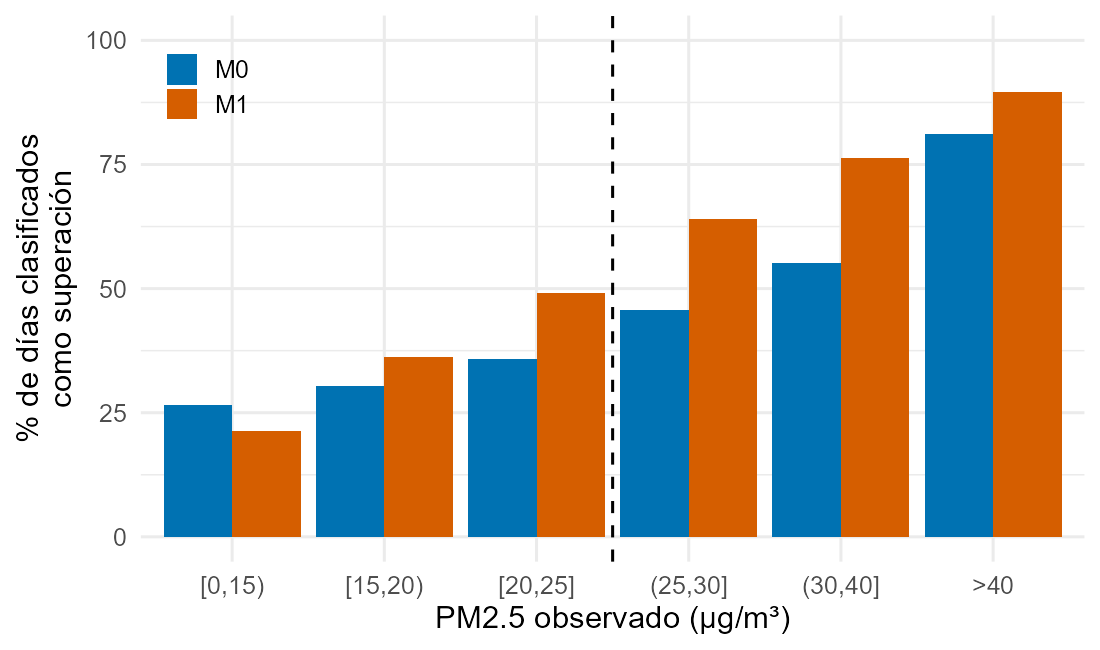
\includegraphics[width=0.58\textwidth]{figuras/errores_magnitud_informe.png}
\caption{Porcentaje de días-estación clasificados como superación según el PM2.5 observado, para M0 y M1 (prueba 2024–2025, n = 6\,863). Por debajo de 25\ugm{} son falsas alarmas y por encima, detecciones.}
\label{fig:magnitud}
\end{figure}

La Figura~\ref{fig:linealidad} respalda la revisión de la linealidad de la Sección~\ref{sec:logistica}: la temperatura, la rapidez del viento y la humedad se apartan de la recta, y la presión y la lluvia casi no. La Figura~\ref{fig:cortes} muestra que, al subir el corte, la sensibilidad baja más rápido de lo que sube el valor predictivo positivo (Sección~\ref{sec:umbral}).

\begin{figure}[H]
\centering
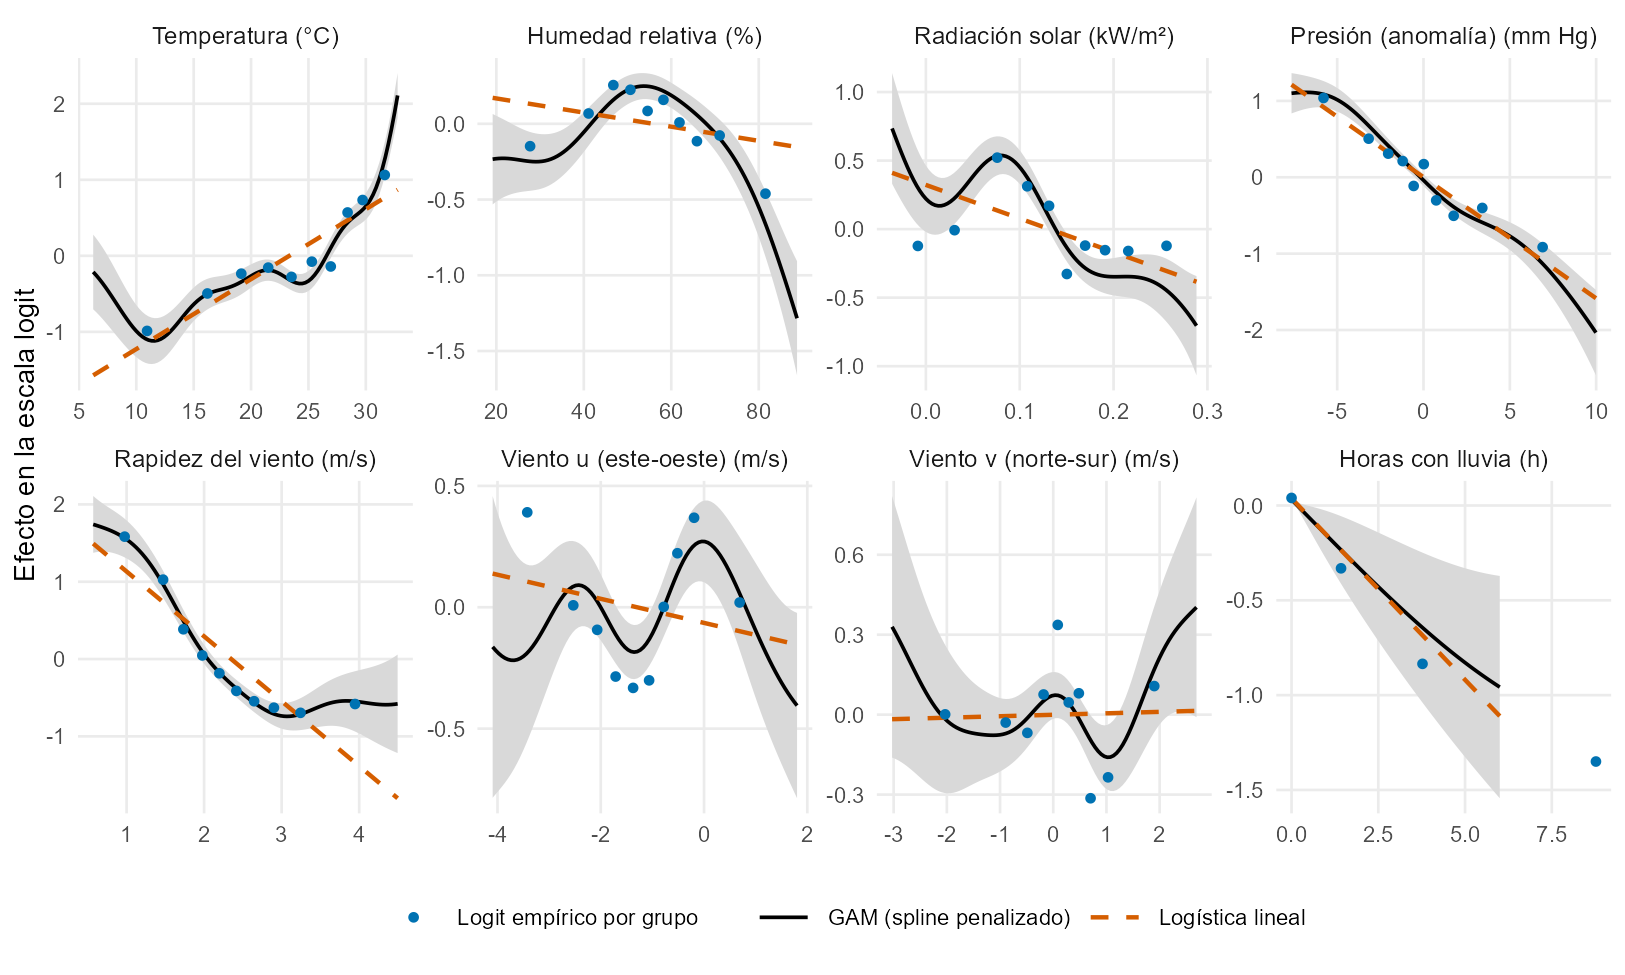
\includegraphics[width=0.95\textwidth]{figuras/linealidad_logit_informe.png}
\caption{Linealidad en la escala logit de las ocho variables meteorológicas en M1 logístico (entrenamiento 2021–2023, n = 10\,965): función del GAM con banda de ± 2 errores estándar (calculada bajo independencia, por lo que es demasiado estrecha), término lineal de la logística y logits empíricos por decil (en la lluvia, días sin lluvia y cuartiles de los días con lluvia), ajustados por estación, temporada y las demás variables. Las curvas están centradas: solo importa su forma.}
\label{fig:linealidad}
\end{figure}

\begin{figure}[H]
\centering
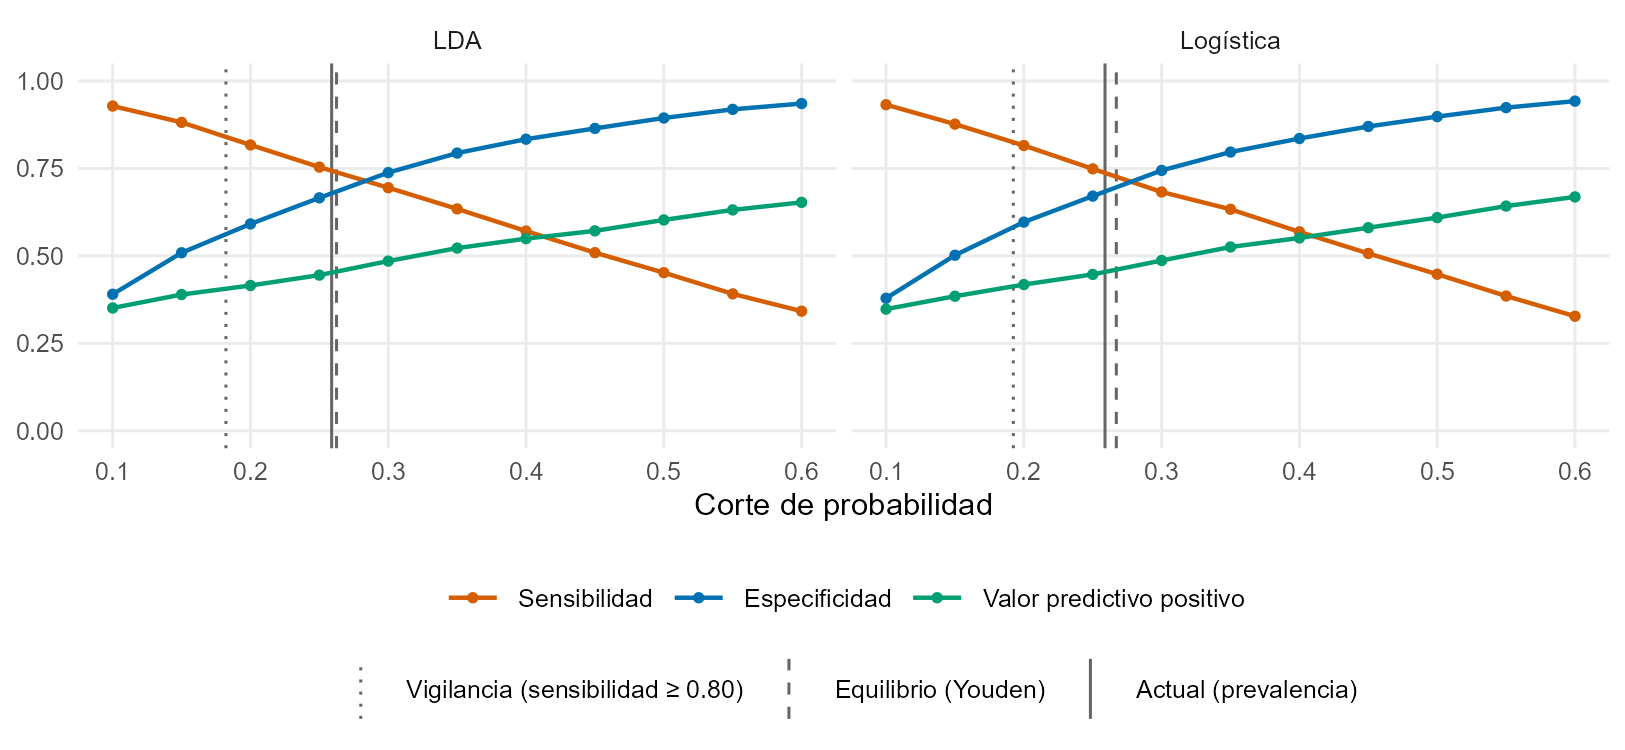
\includegraphics[width=0.95\textwidth]{figuras/metricas_por_corte_informe.png}
\caption{Sensibilidad, especificidad y valor predictivo positivo de M1 en la prueba 2024–2025 (n = 6\,863) según el corte de probabilidad, con los tres cortes elegidos sin usar la prueba (Sección~\ref{sec:umbral}).}
\label{fig:cortes}
\end{figure}

\begin{table}[H]
\centering\small
\caption{Errores de M1 por estación en la prueba 2024–2025 (corte 0.259): días, porcentaje de superación, sensibilidad, especificidad y razón entre el error cuadrático observado y el esperado. † NO2 incluye 272 días del periodo con PM2.5 anómalo (enero de 2024–enero de 2025), sin ninguna superación.}
\label{tbl:c-errores}
\begin{tabular}{lrrrrr}
\toprule
Estación & Días & \% superación & Sensibilidad & Especificidad & Error observado / esperado\\
\midrule
NO & 51 & 49.0 & 0.84 & 0.54 & 1.00\\
SE2 & 705 & 42.8 & 0.95 & 0.25 & 0.90\\
SO & 521 & 39.3 & 0.91 & 0.38 & 1.00\\
NE2 & 218 & 37.2 & 0.85 & 0.51 & 1.05\\
CE & 592 & 30.9 & 0.83 & 0.53 & 1.05\\
NE & 657 & 30.7 & 0.78 & 0.74 & 0.99\\
NTE2 & 670 & 27.3 & 0.69 & 0.82 & 1.13\\
SO2 & 566 & 26.5 & 0.41 & 0.76 & 1.49\\
SE3 & 577 & 25.1 & 0.73 & 0.66 & 1.17\\
NTE & 662 & 16.6 & 0.54 & 0.83 & 1.11\\
SE & 569 & 16.5 & 0.61 & 0.83 & 1.08\\
NO2† & 538 & 11.2 & 0.52 & 0.66 & 0.94\\
SUR & 537 & 11.0 & 0.34 & 0.88 & 1.04\\
\bottomrule
\end{tabular}
\end{table}

La Tabla~\ref{tbl:c-errores} muestra que, con un solo corte para toda la red, el modelo detecta casi todas las superaciones donde son frecuentes (SE2, SO) a costa de muchas falsas alarmas, y pierde muchas donde son raras (SUR) y en SO2. En NO2, la superación baja no es solo una característica del sitio: la mitad de sus días de prueba cae en el periodo con PM2.5 anómalo, sin ninguna superación (22.6\,\% en el resto). Es la razón de recomendar cortes por estación, una vez resuelto el caso de NO2. El error supera al esperado sobre todo en SO2 (1.49) y SE3 (1.17).

\begin{table}[H]
\centering\small
\caption{Calibración de M1 en la prueba 2024–2025: probabilidad media y frecuencia observada de superación por decil de probabilidad.}
\label{tbl:c-calibracion}
\begin{tabular}{lrrrrrrrrrr}
\toprule
Decil & 1 & 2 & 3 & 4 & 5 & 6 & 7 & 8 & 9 & 10\\
\midrule
Probabilidad media & 0.02 & 0.05 & 0.08 & 0.12 & 0.18 & 0.25 & 0.32 & 0.43 & 0.58 & 0.79\\
Frecuencia observada & 0.02 & 0.06 & 0.09 & 0.13 & 0.22 & 0.23 & 0.29 & 0.39 & 0.50 & 0.70\\
\bottomrule
\end{tabular}
\end{table}

\begin{table}[H]
\centering\small
\caption{Recalibración de M1 por temporada en la prueba (regresión logística de la superación sobre el logit de la probabilidad; ideal: intercepto 0 y pendiente 1).}
\label{tbl:c-cal-temporada}
\begin{tabular}{lrrrrr}
\toprule
Temporada & Días & Probabilidad media & Frecuencia observada & Intercepto & Pendiente\\
\midrule
Seca-fría (nov–feb) & 2\,372 & 0.41 & 0.36 & −0.34 & 0.76\\
Seca-cálida (mar–may) & 1\,693 & 0.36 & 0.40 & 0.08 & 0.75\\
Lluvias (jun–oct) & 2\,798 & 0.12 & 0.10 & −0.81 & 0.69\\
\bottomrule
\end{tabular}
\end{table}

La Tabla~\ref{tbl:c-calibracion} y la Tabla~\ref{tbl:c-cal-temporada} muestran que las probabilidades de M1 ordenan bien los días (la frecuencia observada crece con el decil), pero son demasiado extremas: la pendiente de la recalibración es menor que 1 en las tres temporadas.

\begin{table}[H]
\centering\small
\caption{Días-estación por año en el modelado: muestra de la etapa 3 (datos-v1.2) frente al análisis final de la etapa 4 (base v2).}
\label{tbl:c-dias}
\begin{tabular}{lrrr}
\toprule
Año & Etapa 3 & Etapa 4 & Diferencia\\
\midrule
2021 & 2\,863 & 2\,729 & −134\\
2022 & 3\,802 & 4\,218 & 416\\
2023 & 3\,505 & 4\,018 & 513\\
2024 & 2\,894 & 3\,639 & 745\\
2025 & 2\,326 & 3\,224 & 898\\
\bottomrule
\end{tabular}
\end{table}

La Tabla~\ref{tbl:c-dias} muestra que la base final gana días en todos los años salvo 2021, donde los días previos a las reubicaciones salen del entrenamiento (D23). La Figura~\ref{fig:c-no2} respalda la pregunta para SIMA sobre el equipo de PM2.5 de NO2, y la Figura~\ref{fig:c-coef} completa la Figura~\ref{fig:coef} con las indicadoras de estación: SO es la única con un efecto estable mayor que el de CE (la referencia), y el de SE2 no se distingue del de CE.

\begin{figure}[H]
\centering
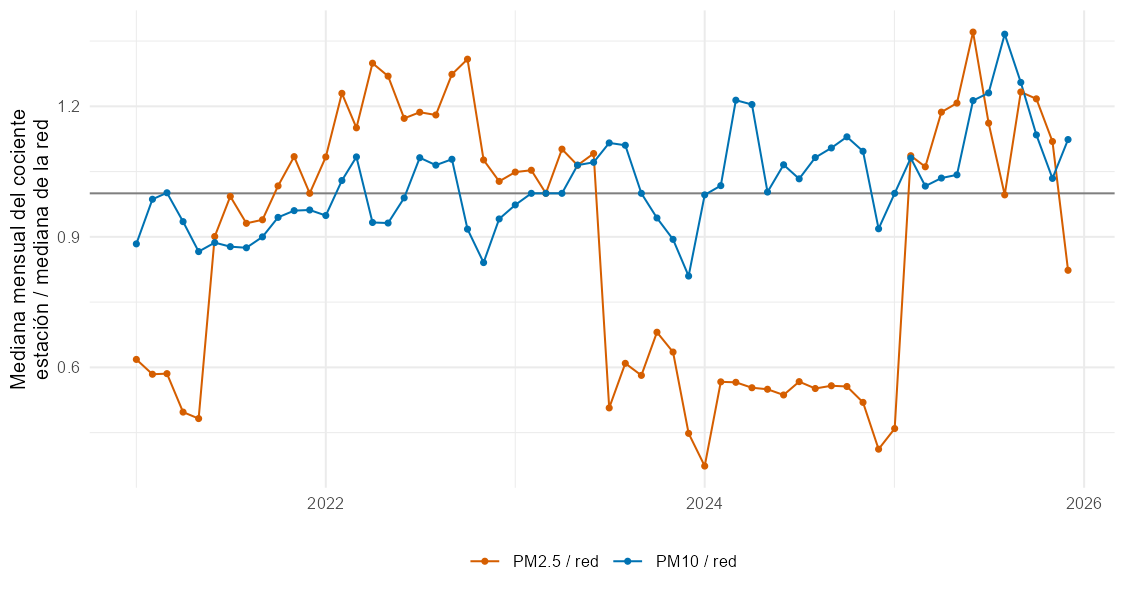
\includegraphics[width=0.75\textwidth]{figuras/no2_relativo_informe.png}
\caption{PM2.5 y PM10 de NO2 (García) divididos entre la mediana de la red, por mes, 2021–2025. El PM2.5 baja a la mitad mientras el PM10 sigue en su nivel, lo que apunta a un problema del equipo de PM2.5.}
\label{fig:c-no2}
\end{figure}

\begin{figure}[H]
\centering
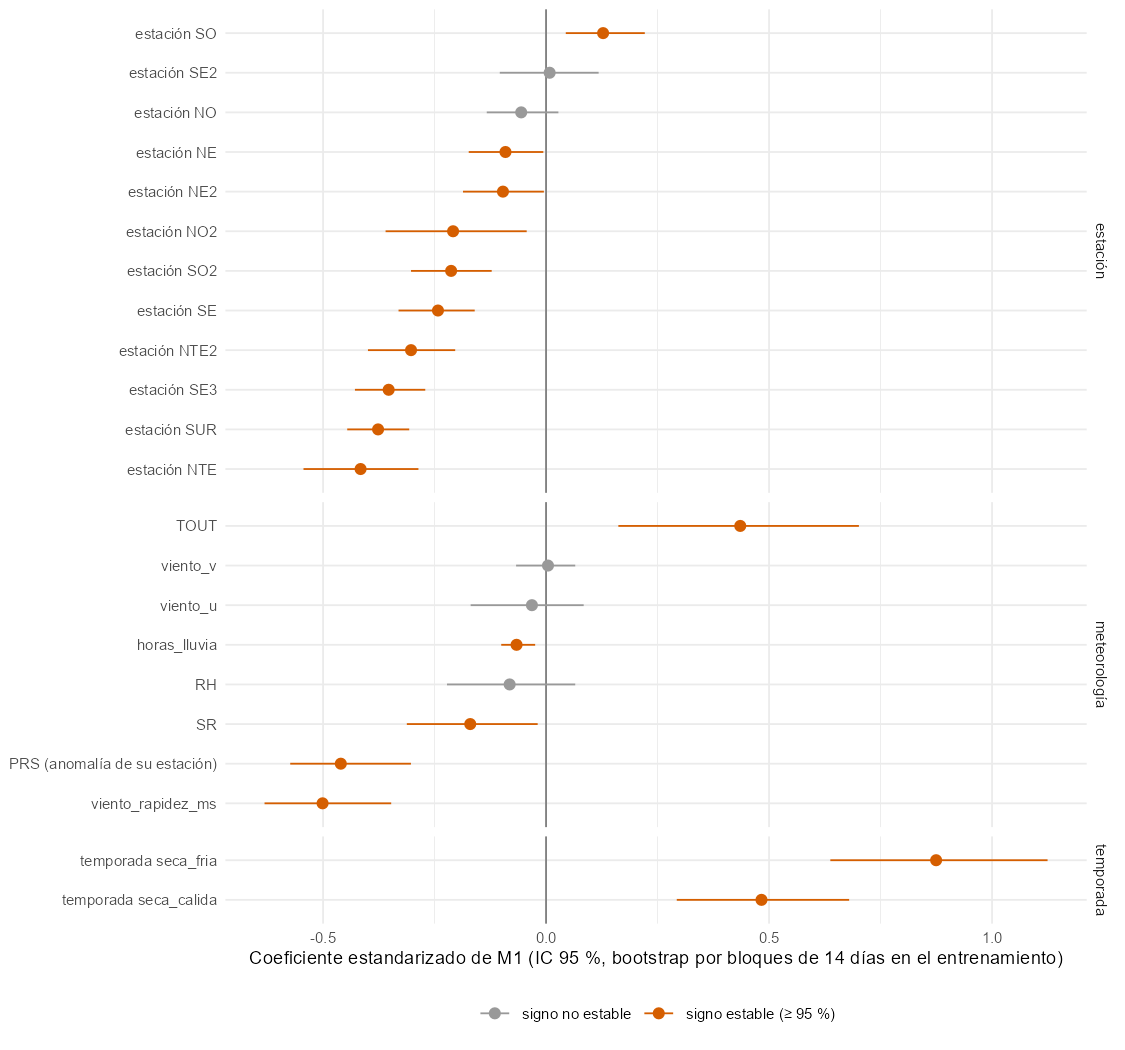
\includegraphics[width=0.78\textwidth]{figuras/coeficientes_ic_informe.png}
\caption{Coeficientes estandarizados de M1 con todas las indicadoras de estación, e IC 95\,\% por bootstrap por bloques de 14 días en el entrenamiento (1\,000 réplicas).}
\label{fig:c-coef}
\end{figure}

% ----------------------- ANEXO D -----------------------
\anexo{Anexo D. Declaratoria de uso de IA (Opción B)}
\begin{itemize}
\item \textbf{Herramientas:} Claude (Anthropic): Claude Opus y Claude Code; ChatGPT y Codex (OpenAI).
\item \textbf{Uso realizado:}
  \begin{itemize}
  \item Claude Opus: planeación de cada etapa, búsqueda y verificación de literatura, decisiones de análisis propuestas, revisión de resultados, redacción de los informes, verificación de los hallazgos de la auditoría final y conversión de este informe a LaTeX.
  \item Claude Code: scripts de R de limpieza, imputación, modelos, validaciones y figuras (\texttt{scripts/02} a \texttt{10}), aplicación Shiny, armado del documento en Quarto y verificación de cifras y citas.
  \item Codex: revisiones independientes de código y cifras de las etapas anteriores, apoyo en la redacción y el formato, preparación de la entrega de la etapa 3 en LaTeX y edición de esta declaratoria a partir de las aportaciones confirmadas por el equipo.
  \item Uso por integrantes: Leonardo Orozco coordinó el trabajo con Claude Opus, Claude Code y Codex para discutir el análisis, desarrollar y revisar el código, contrastar observaciones y preparar los informes. Ignacio Kume utilizó herramientas de IA con razonamiento en profundidad para desarrollar preguntas que el equipo empleó para complementar la exposición y distintas partes del reto. Pablo Alonso Robles Nava utilizó Claude como apoyo analítico para realizar auditorías recurrentes del trabajo y preparar la presentación final. En etapas anteriores, integrantes del equipo también utilizaron Claude y ChatGPT para los borradores de contexto y las fichas de lectura a partir de los PDF de las fuentes.
  \end{itemize}
\item \textbf{Secciones:} todo el informe y el código del repositorio.
\item \textbf{Validación realizada por los estudiantes:} a lo largo del proyecto, Leonardo Orozco contrastó cifras con los CSV, ejecutó el cuaderno de auditoría, revisó las decisiones de modelado y probó la interfaz. Ignacio Kume y Daniel Ayala leyeron los artículos correspondientes a sus fichas; Ignacio verificó fuentes del contexto ambiental y probó la interfaz, y Daniel revisó que el banco de preguntas fuera coherente con los resultados. Pablo Alonso Robles Nava revisó la redacción, investigó el fundamento de los métodos estadísticos y participó en la interpretación de los resultados. Las preguntas desarrolladas por Ignacio y las auditorías coordinadas por Pablo apoyaron la revisión del trabajo y la preparación de la exposición. Estas aportaciones no implican que cada integrante haya reproducido por separado todos los cálculos del informe final.
\item El equipo asume la responsabilidad sobre el contenido entregado, sus decisiones metodológicas, sus citas y sus limitaciones. La asistencia de IA no sustituye la revisión del equipo ni constituye por sí misma una validación de los resultados.
\end{itemize}
